%%%%%%%%%%%%%%%%%%%%%%% 需求分析 %%%%%%%%%%%%%%%%%%%%%%%%%%%%%%%%%%%%%%%%%%
\chapter{需求分析}

\label{cha:demand_analysis}
\section{问题陈述}


我们分析并实现一个连接微供应商和订购商之间的一个中间平台“鲜天下”。通过该平台,我们得以实现这样的目标:聚合小生厂商的生产力以满足大厂家的订单需求,规模化效应减少运行成本,通过可靠的授信模型为小生厂商提供合适额度的贷款以解决成本问题。
% TODO :社会背景

在订购商对虾有较大的需求时,通过“鲜天下”平台,订购商能够在该平台发起订单并支付定金,并实时查看该订单的提交情况与完成情况,如果订单被平台所接受并完成,订购商需要向平台支付剩余款项。

微供应商可以在“鲜天下”平台上注册申请成为认证微供应商,并能够从平台中获得订单。完成订单后,还能够从平台中得到相应款项。同时,根据自己需要,微供应商还可以从“鲜天下”平台申请不超过信用额度的贷款,以此来解决成本问题。

为确保微供应商与订购商之间的协作安全,平台管理人员会对平台所接收到的来自订购商的订单进行审核,并确定是否接受该订单。若接受该订单,平台需要将该订单拆分成多个小订单,并且推送给合适的小生产商在规定时间内完成。同时,平台还需要监控微供应商完成情况,并及时收取货物并完成订购商的订单要求。为了减少微供应商的生产压力,鼓励更多的微供应商参与到该平台中贡献生产力并获得更高的利润,该平台还会记录微供应商相关数据,并根据这些数据,智能地判断每个微供应商可得到的信用额度,以让微供应商获得贷款,减缓它们的资金压力,释放更多的生产力,同时保证平台资金流的安全与稳定。

“鲜天下”平台将采用B/S架构,运行Unix服务器上,能够自动处理用户的请求,并将相关信息存储于数据库中。由于这些信息涉及订单与资金流,该数据库系统必须保证内部数据的一致性,以保证平台的资金流正常运转。


\section{用例析取}

% TODO: 需要修改图片,去做申请额度
% TODO: 简化

对“鲜天下”平台,我们完成了用例图,图示见\autoref{fig:usecase-main}。

%\usepackage{changepage}
%\usepackage{rotating}
%\usepackage{float}
%\usepackage[section]{placeins}
%\begin{sidewaystable}[!Htp]
\begin{figure}[htp]
    %\begin{adjustwidth}{-1.5cm}{-1cm}
    \centering
    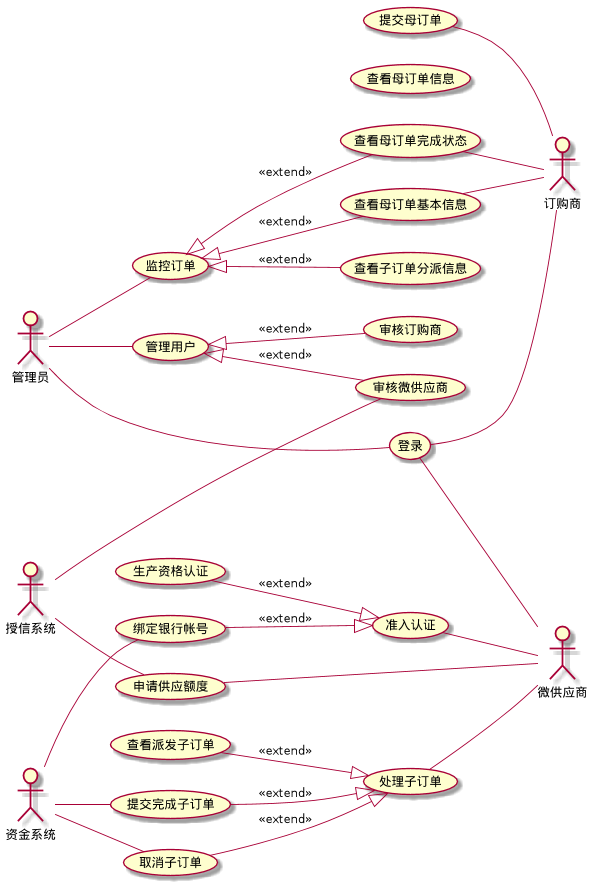
\includegraphics[width=17cm]{figure/usecase/uc_main_ver1.png}
    \caption{“鲜天下”用例图}
    \label{fig:usecase-main}
    %\end{adjustwidth}
\end{figure}


\section{用例规约}

\subsection{登录用例的用例规约}

%\usepackage{changepage}
%\usepackage{rotating}
%\usepackage{float}
%\usepackage[section]{placeins}
%\begin{sidewaystable}[!Htp]
    \begin{figure}[htp]
        %\begin{adjustwidth}{-1.5cm}{-1cm}
        \centering
        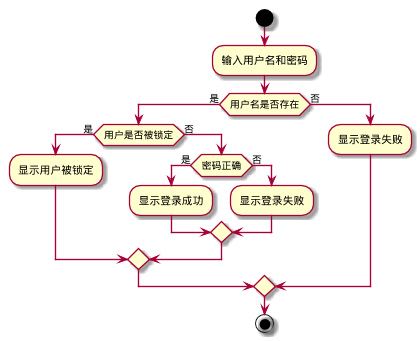
\includegraphics[width=12cm]{figure/usecase/uc_sub/uc_login.png}
        \caption{登录用例-活动图}
        \label{fig:logon-uml}
        %\end{adjustwidth}
    \end{figure}
    

\begin{enumerate}
	\item \textbf{简要说明}  \\ 本用例描述订购商/微供应商/管理员如何登录到鲜天下平台。
	\item \textbf{参与者} \\ 订购商、微供应商、管理员, 以下简称用户
	\item \textbf{事件流} \\ 相应活动图可见\autoref{fig:logon-uml}。
	\begin{enumerate} 
        \item \textbf{基本事件流} \\ 本用例开始于用户希望登录到鲜天下平台。
        \begin{enumerate}
            \item 系统请求用户输入用户名和密码。
            \item 用户输入用户名和密码。
            \item 系统验证用户输入的用户名和密码。
            \begin{enumerate}
                \item 用户名不存在。
                \item 用户被锁定。
                \item 用户名对应的密码不正确。
            \end{enumerate}
            \item 用户成功登录到主界面并进行其它操作。
        \end{enumerate}
        \item \textbf{后备事件流}
        \begin{enumerate}
            \item 用户名不存在。
            \begin{enumerate}
                \item 系统显示错误信息 “用户名不存在或密码错误, 超过5次后锁定”。
                \item 返回事件流第一步。
            \end{enumerate}
            \item 用户被锁定。
            \begin{enumerate}
                \item 系统显示错误信息 “用户被锁定, 请联系客服申诉处理”。
                \item 返回事件流第一步。
            \end{enumerate}
            \item 用户名对应的密码不正确。
            \begin{enumerate}
                \item 系统显示错误信息 “用户名不存在或密码错误, 超过5次后锁定”。
                \item 系统将用户错误的登录尝试次数 +1。
                \item 检查登录尝试次数是否超过上限, 超过则锁定用户并发送通知短信。
                \item 返回事件流第一步。
            \end{enumerate}
        \end{enumerate}
    \end{enumerate}
    \item \textbf{特殊需求} \\ 密码输入框必须以密文方式呈现。
    \item \textbf{前置条件} \\ 用例开始前, 用户需要打开对应的系统登录界面, 且用户处于未登录状态。
    \item \textbf{后置条件} \\ 如果用例成功, 系统状态转换为登录态;若失败, 系统状态不改变。
\end{enumerate}


\subsection{提交母订单用例的用例规约}



\begin{enumerate}
	\item \textbf{简要说明}  \\ 本用例描述订购商如何向鲜天下平台提交新订单。
	\item \textbf{参与者} \\ 订购商。
	\item \textbf{事件流} \\ 相应活动图可见\autoref{fig:put-order-uml}。
	\begin{enumerate} 
        \item \textbf{基本事件流} \\ 本用例开始于处于登录态的订购商向鲜天下平台申请订购货物。
        \begin{enumerate}
            \item 用户输入需要虾的数量, 配送地点和配送方式。 \\ 
            选择配送地点过程为:系统显示可选地点列表, 用户依次点选省, 市, 区, 系统显示的可选地点列表层级也从省,下降到是市,最后到区。 用户最后需手动输入街道地址。系统会在用户的输入面板上方列出用户使用的过往完整地址,
            用户可以点击历史地址来一次性完成地址输入。 \\ 
            选择配送方式为点选系统提供的几种可选配送方式之一,选择后配送方式其它选项变为不可选状态。
            \item 系统检测用户的输入是否合法。
            \begin{enumerate}
                \item 客户请求的虾数量不在余量范围内。
                \item 客户没有输入完整的地址。
                \item 客户没有选择配送方式。
            \end{enumerate}
            \item 用户选择确认当前信息继续进行预约或取消交易。
            \begin{enumerate}
                \item 用户选择取消。
            \end{enumerate}
            \item 用户选择订金交付方式。 \\ 选项包括: 立即交付定金, 请求人工面谈.
            \begin{itemize}
                \item 若用户选择立即交付定金, 则转入支付页面, 填写支付信息(如稅号和公司抬头等)。
                \item 若用户选择请求人工面谈, 则请求用户填写公司联系人信息并预约会谈时间。
                \item 用户也可选择取消。
            \end{itemize}
            \item 预订结束, 订单被提交
        \end{enumerate}
        \item \textbf{后备事件流}
        \begin{enumerate}
            \item 客户请求的虾数量不在余量范围内。
            \begin{enumerate}
                \item 系统显示错误信息 “您申请的商品余量不足”。
                \item 返回事件流第一步。
            \end{enumerate}
            \item 客户没有输入完整的地址。
            \begin{enumerate}
                \item 系统显示错误信息 “您没有输入完整的地址”。
                \item 返回事件流第一步。
            \end{enumerate}
            \item 客户没有选择配送方式。
            \begin{enumerate}
                \item 系统显示错误信息 “您没有选择配送方式”。
                \item 返回事件流第一步。
            \end{enumerate}
            \item 在确定信息或选择定金交付方式时,用户选择取消。
            \begin{enumerate}
                \item 返回事件流第一步。
            \end{enumerate}
        \end{enumerate}
    \end{enumerate}
    \item \textbf{特殊需求} \\ 无。
    \item \textbf{前置条件} \\ 用例开始前, 用户需要处于已登录状态下, 并打开交易界面。
    \item \textbf{后置条件} \\ 如果用例成功,用户提交的订单被保存为预订态或取消态,预订态的订单需保存在数据库中,取消态的订单直接丢弃,在接受到用户的定金转账后 (无论是立即交付定金/人工面谈后交付定金),订单状态均切换为待完成态。
\end{enumerate}



%\usepackage{changepage}
%\usepackage{rotating}
%\usepackage{float}
%\usepackage[section]{placeins}
%\begin{sidewaystable}[!Htp]
    \begin{figure}[htp]
        %\begin{adjustwidth}{-1.5cm}{-1cm}
        \centering
        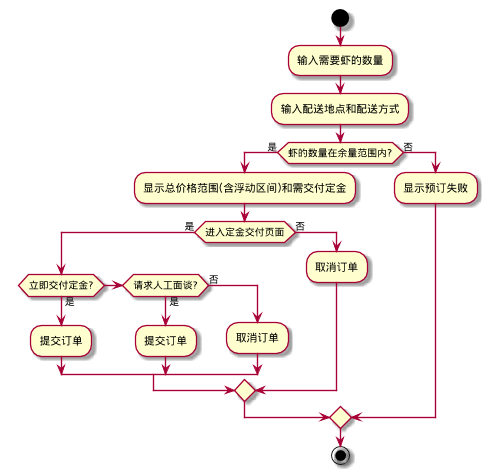
\includegraphics[width=0.7\textwidth]{figure/usecase/uc_sub/uc_client_submit_request.png}
        \caption{提交母订单用例-活动图}
        \label{fig:put-order-uml}
        %\end{adjustwidth}
    \end{figure}
    
\subsection{查看母订单信息用例的用例规约}

% TODO: wyf


\begin{enumerate}
	\item \textbf{简要说明}  \\ 本用例描述订购商或管理员如何查看订单的信息。
	\item \textbf{参与者} \\ 订购商,管理员。
	\item \textbf{事件流} \\ 相应活动图可见\autoref{fig:watch-order-umls}。
	\begin{enumerate} 
        \item \textbf{基本事件流} \\ 本用例开始于处于登录态的订购商或管理员向鲜天下平台请求订单信息。
        \begin{enumerate}
            \item 系统读取用户设置的订单过滤器的值。
            \item 系统向平台发送过滤器, 平台返回相关订单状态。
            \item 系统显示订单数据。
        \end{enumerate}
    \end{enumerate}
    \item \textbf{特殊需求} \\ 无。
    \item \textbf{前置条件} \\ 用例开始前, 用户需要处于已登录状态下, 并打开订单信息界面, 同时刚刚执行了一次请求指令。
    \item \textbf{后置条件} \\ 无。
\end{enumerate}



%\usepackage{changepage}
%\usepackage{rotating}
%\usepackage{float}
%\usepackage[section]{placeins}
%\begin{sidewaystable}[!Htp]
    \begin{figure}[htp]
        %\begin{adjustwidth}{-1.5cm}{-1cm}
        \centering
        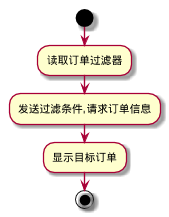
\includegraphics[width=0.4\textwidth]{figure/usecase/uc_sub/uc_client_or_admin_view_request.png}
        \caption{查看母订单用例-活动图}
        \label{fig:watch-order-uml}
        %\end{adjustwidth}
    \end{figure}
    

\subsection{查看子订单分派信息用例的用例规约}

% TODO: wyf




\begin{enumerate}
	\item \textbf{简要说明}  \\ 本用例描述管理员如何查看子订单的分派信息。
	\item \textbf{参与者} \\ 管理员。
	\item \textbf{事件流} \\ 相应活动图可见\autoref{fig:watch-order-devide-uml}。
	\begin{enumerate} 
        \item \textbf{基本事件流} \\ 本用例开始于处于登录态的订购商或管理员向鲜天下平台请求订单信息。
        \begin{enumerate}
            \item 系统读取用户设置的订单过滤器的值。
            \item 系统向平台发送过滤器, 平台返回相关订单状态。
            \item 系统根据过滤器筛选订单并显示。
        \end{enumerate}
    \end{enumerate}
    \item \textbf{特殊需求} \\ 无。
    \item \textbf{前置条件} \\ 用例开始前, 用户需要处于已登录状态下, 并打开订单信息界面, 同时刚刚执行了一次请求指令。
    \item \textbf{后置条件} \\ 无。
\end{enumerate}



%\usepackage{changepage}
%\usepackage{rotating}
%\usepackage{float}
%\usepackage[section]{placeins}
%\begin{sidewaystable}[!Htp]
    \begin{figure}[htp]
        %\begin{adjustwidth}{-1.5cm}{-1cm}
        \centering
        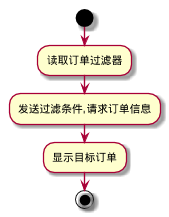
\includegraphics[width=0.4\textwidth]{figure/usecase/uc_sub/uc_admin_view_dispatch.png}
        \caption{查看子订单分派用例-活动图}
        \label{fig:watch-order-devide-uml}
        %\end{adjustwidth}
    \end{figure}
    

\subsection{审核订购商用例的用例规约}

% TODO: tl


\begin{enumerate}
	\item \textbf{简要说明}  \\ 本用例描述管理员如何审核订购商的资质。
	\item \textbf{参与者} \\ 管理员。
	\item \textbf{事件流} \\ 相应活动图可见\autoref{fig:shenhe-order-uml}。
	\begin{enumerate} 
        \item \textbf{基本事件流} \\ 本用例开始于处于登录态的管理员向鲜天下请求待检查的订购商队列。
        \begin{enumerate}
            \item 系统读取待检查的订购商队列。
            \item 系统读取管理员选择的订购商并显示信息。
            \item 系统请求管理员决定是否通过。
            \begin{enumerate}
                \item 若管理员同意通过,则将订购商帐号标记为验证通过, 同时向订购商填写的邮件地址发送验证成功邮件。
                \item 若管理员否决, 则将订购商帐号标记为验证不通过, 同时向订购商填写的邮件地址发送验证失败邮件。
            \end{enumerate}
            \item 从队列中移除订购商请求, 回到第一步。
        \end{enumerate}
    \end{enumerate}
    \item \textbf{特殊需求} \\ 无。
    \item \textbf{前置条件} \\ 用例开始前, 管理员需要处于已登录状态下, 并打开订购商信息界面。
    \item \textbf{后置条件} \\ 无。
\end{enumerate}



%\usepackage{changepage}
%\usepackage{rotating}
%\usepackage{float}
%\usepackage[section]{placeins}
%\begin{sidewaystable}[!Htp]
    \begin{figure}[htp]
        %\begin{adjustwidth}{-1.5cm}{-1cm}
        \centering
        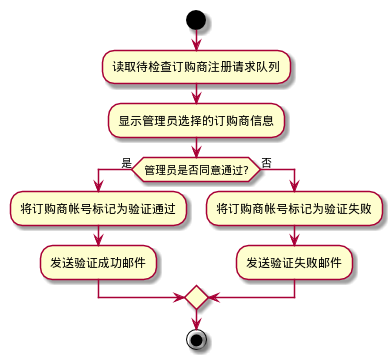
\includegraphics[width=0.4\textwidth]{figure/usecase/uc_sub/uc_admin_check_client.png}
        \caption{审核订购商用例-活动图}
        \label{fig:shenhe-order-uml}
        %\end{adjustwidth}
    \end{figure}



\subsection{审核微供应商的用例规约}

% TODO: tl



\begin{enumerate}
	\item \textbf{简要说明}  \\ 本用例描述管理员如何审核微供应商的资质。
	\item \textbf{参与者} \\ 管理员。
	\item \textbf{事件流} \\ 相应活动图可见\autoref{fig:shenhe-gongying-uml}。
	\begin{enumerate} 
        \item \textbf{基本事件流} \\ 本用例开始于处于登录态的管理员向鲜天下请求待检查的微供应商队列。
        \begin{enumerate}
            \item 系统读取待检查的微供应商队列。
            \item 系统读取管理员选择的微供应商并显示信息。
            \item 系统请求管理员决定是否通过。
            \begin{enumerate}
                \item 若管理员同意通过,则将微供应商帐号标记为验证通过,同时向微供应商填写的邮件地址发送验证成功邮件。
                \item 若管理员否决,则将微供应商帐号标记为验证不通过,同时向订购商填写的邮件地址发送验证失败邮件。
            \end{enumerate}
            \item 从队列中移除微供应商请求, 回到事件流第一步。
        \end{enumerate}
    \end{enumerate}
    \item \textbf{特殊需求} \\ 无。
    \item \textbf{前置条件} \\ 用例开始前, 管理员需要处于已登录状态下, 并打开微供应商信息界面。
    \item \textbf{后置条件} \\ 无。
\end{enumerate}



%\usepackage{changepage}
%\usepackage{rotating}
%\usepackage{float}
%\usepackage[section]{placeins}
%\begin{sidewaystable}[!Htp]
    \begin{figure}[htp]
        %\begin{adjustwidth}{-1.5cm}{-1cm}
        \centering
        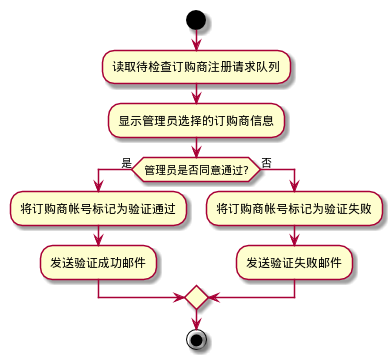
\includegraphics[width=0.4\textwidth]{figure/usecase/uc_sub/uc_admin_check_client.png}
        \caption{审核微供应商用例-活动图}
        \label{fig:shenhe-gongying-uml}
        %\end{adjustwidth}
    \end{figure}


\subsection{生产资格认证用例的用例规约}

% TODO: tl



\begin{enumerate}
	\item \textbf{简要说明}  \\ 本用例描述微供应商如何申请生产资格认证。
	\item \textbf{参与者} \\ 微供应商。
	\item \textbf{事件流} \\ 相应活动图可见\autoref{fig:uc_provider_request_check-uml}。
	\begin{enumerate} 
        \item \textbf{基本事件流} \\ 本用例开始于处于登录态的微供应商向鲜天下申请生产资格认证。
        \begin{enumerate}
            \item 检查用户是否已经经过验证和是否有处理中的验证。
            \begin{enumerate}
                \item 尚未验证且没有处理中的验证。
                \item 其它。
            \end{enumerate}
        \end{enumerate}
        \item \textbf{后备事件流}
        \begin{enumerate}
            \item 若满足条件。
            \begin{enumerate}
                \item 请求微供应商输入验证信息。
                \item 将请求发送到平台。
                \item 平台将请求分派到活动管理员。
                \item 将用户标记为验证处理中。
            \end{enumerate}
            \item 若不满足条件。
            \begin{enumerate}
                \item 显示申请失败和申请失败的原因。
            \end{enumerate}
        \end{enumerate}
    \end{enumerate}
    \item \textbf{特殊需求} \\ 无。
    \item \textbf{前置条件} \\ 用例开始前, 微供应商需要处于已登录状态下, 并打开微供应商申请验证界面。
    \item \textbf{后置条件} \\ 无。
\end{enumerate}



%\usepackage{changepage}
%\usepackage{rotating}
%\usepackage{float}
%\usepackage[section]{placeins}
%\begin{sidewaystable}[!Htp]
    \begin{figure}[htp]
        %\begin{adjustwidth}{-1.5cm}{-1cm}
        \centering
        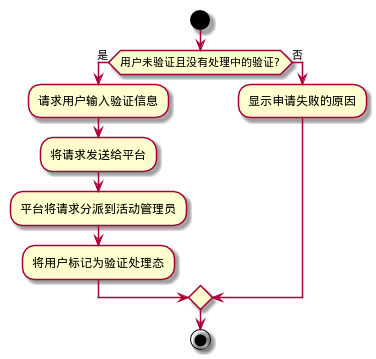
\includegraphics[width=0.7\textwidth]{figure/usecase/uc_sub/uc_provider_request_check.png}
        \caption{生产资格认证用例-活动图}
        \label{fig:uc_provider_request_check-uml}
        %\end{adjustwidth}
    \end{figure}


\subsection{购买资格认证用例的用例规约}

% TODO: 填写增加生产力




\begin{enumerate}
	\item \textbf{简要说明}  \\ 本用例描述微供应商如何申请生产资格认证。
	\item \textbf{参与者} \\ 微供应商。
	\item \textbf{事件流} \\ 相应活动图可见\autoref{fig:uc_client_request_check}。
	\begin{enumerate} 
        \item \textbf{基本事件流} \\  本用例开始于处于登录态的订购商向鲜天下申请购买资格认证。
        \begin{enumerate}
            \item 检查用户是否已经经过验证和是否有处理中的验证。
            \begin{enumerate}
                \item 尚未验证且没有处理中的验证。
                \item 其它。
            \end{enumerate}
        \end{enumerate}
        \item \textbf{后备事件流}
        \begin{enumerate}
            \item 尚未验证且没有处理中的验证。
            \begin{enumerate}
                \item 请求订购商输入验证信息。
                \item 将请求发送到平台。
                \item 平台将请求分派到活动管理员。
                \item 将用户标记为验证处理中。
            \end{enumerate}
            \item 其他情况。
            \begin{enumerate}
                \item 显示申请失败和申请失败的原因。
            \end{enumerate}
        \end{enumerate}
    \end{enumerate}
    \item \textbf{特殊需求} \\ 无。
    \item \textbf{前置条件} \\ 用例开始前, 订购商需要处于已登录状态下, 并打开订购商申请验证界面。
    \item \textbf{后置条件} \\ 无。
\end{enumerate}



%\usepackage{changepage}
%\usepackage{rotating}
%\usepackage{float}
%\usepackage[section]{placeins}
%\begin{sidewaystable}[!Htp]
    \begin{figure}[htp]
        %\begin{adjustwidth}{-1.5cm}{-1cm}
        \centering
        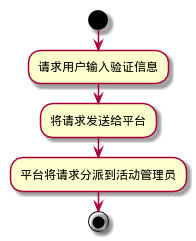
\includegraphics[width=0.4\textwidth]{figure/usecase/uc_sub/uc_client_request_check.png}
        \caption{生产资格认证用例-活动图}
        \label{fig:uc_client_request_check}
        %\end{adjustwidth}
    \end{figure}


\subsection{绑定银行账号用例的用例规约}

% TODO: tl




\begin{enumerate}
	\item \textbf{简要说明}  \\ 本用例描述微供应商如何绑定银行帐号。
	\item \textbf{参与者} \\ 微供应商。
	\item \textbf{事件流} \\ 相应活动图可见\autoref{fig:uc_provider_bind_bank}。
	\begin{enumerate} 
        \item \textbf{基本事件流} \\  本用例开始于处于登录态的微供应商向鲜天下请求绑定银行帐号。
        \begin{enumerate}
            \item 请求用户输入待绑定的银行信息。
            \item 将信息发送到平台进行验证。
            \begin{enumerate}
                \item 支付信息合法。
                \item 支付信息不合法。
            \end{enumerate}
        \end{enumerate}
        \item \textbf{后备事件流}
        \begin{enumerate}
            \item 支付信息合法。
            \begin{enumerate}
                \item 保存支付信息到数据库。
                \item 显示绑定成功。
            \end{enumerate}
            \item 支付信息不合法。
            \begin{enumerate}
                \item 显示绑定失败和绑定失败的原因。
            \end{enumerate}
        \end{enumerate}
    \end{enumerate}
    \item \textbf{特殊需求} \\ 无。
    \item \textbf{前置条件} \\ 用例开始前, 微供应商需要处于已登录状态下, 并打开微供应商银行帐号界面, 且微供应商银行帐号处于未绑定状态。
    \item \textbf{后置条件} \\ 无。
\end{enumerate}



%\usepackage{changepage}
%\usepackage{rotating}
%\usepackage{float}
%\usepackage[section]{placeins}
%\begin{sidewaystable}[!Htp]
    \begin{figure}[htp]
        %\begin{adjustwidth}{-1.5cm}{-1cm}
        \centering
        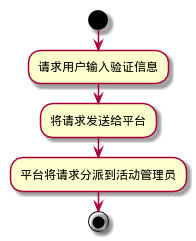
\includegraphics[width=0.4\textwidth]{figure/usecase/uc_sub/uc_client_request_check.png}
        \caption{绑定银行账号用例-活动图}
        \label{fig:uc_provider_bind_bank}
        %\end{adjustwidth}
    \end{figure}



\subsection{申请供应额度用例的用例规约}

% TODO: wyf



\begin{enumerate}
	\item \textbf{简要说明}  \\ 本用例描述微供应商如何申请增加配额。
	\item \textbf{参与者} \\ 微供应商。
	\item \textbf{事件流} \\ 相应活动图可见\autoref{fig:uc_provider_request_quota}。
	\begin{enumerate} 
        \item \textbf{基本事件流} \\  本用例开始于处于登录态的微供应商向鲜天下申请一个配额订单。
        \begin{enumerate}
            \item 请求用户输入所需额度。
            \item 检查请求额度是否小于等于总额度。
            \begin{enumerate}
                \item 请求额度小于等于总额度。
                \item 请求额度大于总额度。
            \end{enumerate}
            \item 请求用户确认。
            \begin{enumerate}
                \item 用户确认。
                \item 用户取消。
            \end{enumerate}
        \end{enumerate}
        \item \textbf{后备事件流}
        \begin{enumerate}
            \item 请求额度小于等于总额度。
            \begin{enumerate}
                \item 转至事件流第三步。
            \end{enumerate}
            \item 请求额度大于总额度。
            \begin{enumerate}
                \item  显示申请失败。
            \end{enumerate}
            \item 用户确认。
            \begin{enumerate}
                \item 扣除申请配额。
                \item 保存订单。
                \item 显示申请成功。
            \end{enumerate}
            \item 用户取消。
            \begin{enumerate}
                \item  显示申请取消。
            \end{enumerate}
        \end{enumerate}
    \end{enumerate}
    \item \textbf{特殊需求} \\ 无。
    \item \textbf{前置条件} \\ 用例开始前, 微供应商需要处于已登录状态下, 并打开微供应商申请配额界面。
    \item \textbf{后置条件} \\ 无。
\end{enumerate}



%\usepackage{changepage}
%\usepackage{rotating}
%\usepackage{float}
%\usepackage[section]{placeins}
%\begin{sidewaystable}[!Htp]
    \begin{figure}[htp]
        %\begin{adjustwidth}{-1.5cm}{-1cm}
        \centering
        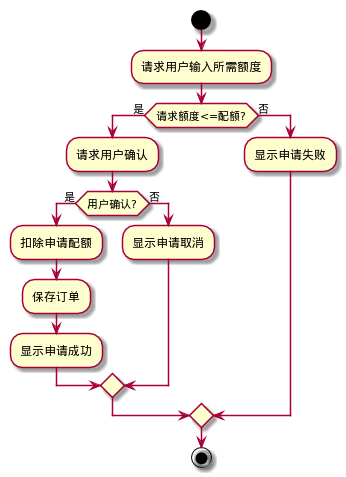
\includegraphics[width=0.5\textwidth]{figure/usecase/uc_sub/uc_provider_request_quota.png}
        \caption{申请供应额度用例-活动图}
        \label{fig:uc_provider_request_quota}
        %\end{adjustwidth}
    \end{figure}




\subsection{查看派发子订单用例的用例规约}

% TODO: tl


\begin{enumerate}
	\item \textbf{简要说明}  \\ 本用例描述微供应商如何查看被分派的子订单。
	\item \textbf{参与者} \\ 微供应商。
	\item \textbf{事件流} \\ 相应活动图可见\autoref{fig:uc_provider_view}。
	\begin{enumerate} 
        \item \textbf{基本事件流} \\ 本用例开始于处于登录态的管理员向鲜天下平台请求订单信息。
        \begin{enumerate}
            \item 用户提交查看订单的请求。
            \item 系统读取分派给微供应商的所有订单。
            \item 系统显示所有订单详情。
        \end{enumerate}
    \end{enumerate}
    \item \textbf{特殊需求} \\ 无。
    \item \textbf{前置条件} \\ 用例开始前, 用户需要处于已登录状态下, 并打开订单信息界面。
    \item \textbf{后置条件} \\ 无。
\end{enumerate}



%\usepackage{changepage}
%\usepackage{rotating}
%\usepackage{float}
%\usepackage[section]{placeins}
%\begin{sidewaystable}[!Htp]
    \begin{figure}[htp]
        %\begin{adjustwidth}{-1.5cm}{-1cm}
        \centering
        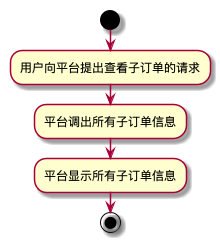
\includegraphics[width=0.4\textwidth]{figure/usecase/uc_sub/uc_provider_view.png}
        \caption{查看派发子订单用例-活动图}
        \label{fig:uc_provider_view}
        %\end{adjustwidth}
    \end{figure}



\subsection{取消子订单用例的用例规约}



\begin{enumerate}
	\item \textbf{简要说明}  \\ 本用例描述微供应商取消被分派订单的流程。
	\item \textbf{参与者} \\ 微供应商、资金系统。
	\item \textbf{事件流} \\ 相应活动图可见\autoref{fig:uc_provider_cancel}。
	\begin{enumerate} 
        \item \textbf{基本事件流} \\ 本用例开始于处于登录态的微供应商向鲜天下平台处理子订单后的界面。
        \begin{enumerate}
            \item 微供应商向平台发送取消子订单的请求。
            \item 平台向资金系统转发请求。
            \item 资金系统同意取消订单。
            \item 在数据库中更改子订单相关信息
        \end{enumerate}
        \item \textbf{后备事件流}
        \begin{enumerate}
            \item 资金系统不同意取消订单。
            \begin{enumerate}
                \item 系统显示错误信息 "订单不满足取消条件,无法取消"。
                \item 退出事件流。
            \end{enumerate}
        \end{enumerate}
    \end{enumerate}
    \item \textbf{特殊需求} \\ 无。
    \item \textbf{前置条件} \\ 用例开始前, 用户需要处于已登录状态下, 并打开订单信息界面, 同时刚刚执行了一次查看子订单请求指令。
    \item \textbf{后置条件} \\ 无。
\end{enumerate}



%\usepackage{changepage}
%\usepackage{rotating}
%\usepackage{float}
%\usepackage[section]{placeins}
%\begin{sidewaystable}[!Htp]
    \begin{figure}[htp]
        %\begin{adjustwidth}{-1.5cm}{-1cm}
        \centering
        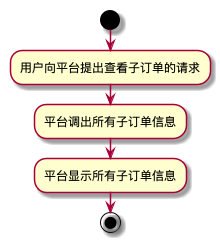
\includegraphics[width=0.4\textwidth]{figure/usecase/uc_sub/uc_provider_view.png}
        \caption{取消子订单用例-活动图}
        \label{fig:uc_provider_cancel}
        %\end{adjustwidth}
    \end{figure}



\subsection{提交完成子订单用例的用例规约}

% TODO: tl



\begin{enumerate}
	\item \textbf{简要说明}  \\ 本用例描述微供应商和资金系统完成子订单的提交。
	\item \textbf{参与者} \\ 微供应商、资金系统。
	\item \textbf{事件流} \\ 相应活动图可见\autoref{fig:uc_provider_commit}。
	\begin{enumerate} 
        \item \textbf{基本事件流} \\ 本用例开始于处于登录态的微供应商向鲜天下平台处理子订单后的界面。
        \begin{enumerate}
            \item 微供应商向平台发送提交子订单的请求。
            \item 平台向资金系统转发请求。
            \item 资金系统确认子订单的提交。
            \item 平台在数据库中更改子订单相关信息(包括子订单、母订单信息)。
        \end{enumerate}
        \item \textbf{后备事件流}
        \begin{enumerate}
            \item 资金系统不同意提交子订单。
            \begin{enumerate}
                \item 系统显示错误信息 "订单不满足提交条件,无法提交"。
                \item 退出事件流。
            \end{enumerate}
        \end{enumerate}
    \end{enumerate}
    \item \textbf{特殊需求} \\ 无。
    \item \textbf{前置条件} \\ 用例开始前, 用户需要处于已登录状态下, 并打处理子订单信息界面,同时刚刚执行了一次查看子订单请求指令。
    \item \textbf{后置条件} \\ 无。
\end{enumerate}



%\usepackage{changepage}
%\usepackage{rotating}
%\usepackage{float}
%\usepackage[section]{placeins}
%\begin{sidewaystable}[!Htp]
    \begin{figure}[htp]
        %\begin{adjustwidth}{-1.5cm}{-1cm}
        \centering
        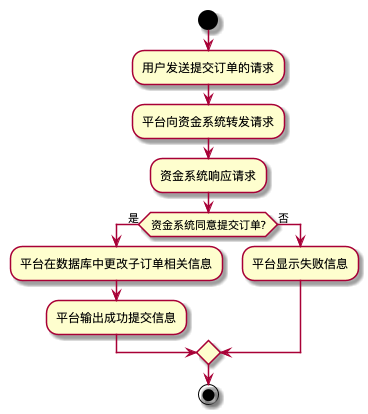
\includegraphics[width=0.4\textwidth]{figure/usecase/uc_sub/uc_provider_commit.png}
        \caption{提交完成子订单用例-活动图}
        \label{fig:uc_provider_commit}
        %\end{adjustwidth}
    \end{figure}


\section{"鲜天下"实现补充规约}
    补充规约列出了不便于在用例模型的用例中获取的系统需求。补充规约用例模型一起记录关于系统的一整套需求。


\subsection{范围}
    \begin{enumerate}

        \item 本补充规约适用于"鲜天下"系统,将要由学习面向对象软件分析与设计的学生开发。
        \item 本规约除定义了在许多用例中所共有的功能性需求以外,还定义了系统的非功能性需求,例如:可靠性、可用性、性能和可支持性等。

    \end{enumerate}

\subsection{功能}
    \begin{enumerate}
        \item 平台能够在管理员进行订单处理时给出可行方案、方便管理员进行订单的拆分和分派。
        \item 供应商在提交订单后违约需要支付支付违约金,接收到订单的微供应商也需要得到补充。
        \item 微生产商注册时将提供生产力相关信息,并默认无条件接受平台的分派,否则注册时应在相关信息填写好所能接受的供货范围与供货量。
    \end{enumerate}


\subsection{可靠性}

    "鲜天下"交易平台应该在每周七天,每天二十四小时内都应是可以使用的。宕机的时间应少于 5\%。配备有2名维护人员,轮流提供维护服务。


\subsection{性能}
    \begin{enumerate}
        \item 通过CDN服务使得服务器的平均响应时间不能超过1秒。
    \end{enumerate}

\subsection{安全性}
    \begin{enumerate}
        \item 通过后端用户输入过滤来防范XSS攻击。
        \item 服务端配置完善的跨域规则,同时利用后端框架提供的CSRF\_TOKEN防范CSRF攻击。
        \item 全站采用HTTPS、密码等不对称加密方式加密后传输防范中间人攻击。
        \item 采用后端框架提供的参数化查询来避免SQL注入攻击。
    \end{enumerate}

\section{术语表}

\begin{table}[h] %voc table result
	\centering
        \label{tab:glossary}
        \caption{“鲜天下”-术语表}
		\begin{tabular}{*{4}{c}}
			\toprule
	 		编号 & 术语 & 含义 & 备注\\
            \midrule
            1 & 微供应商 & 生产虾的微小供应商, 为平台上实际货物的生产者 \\
            2 & 订购商 & 购买虾的订购商, 为平台上实际货物的购买者 \\
            3 & 平台 & 连接微供应商和订购商的桥梁, 负责订单派发, 资金分派, 物流等功能\\
			\bottomrule
		\end{tabular}
\end{table}

